\clearpage
\onecolumn
\begin{landscape}
	\section{Anhang}
	\subsection{Approximation des Bode-Diagramms}\label{approx_bode}
	\renewcommand{\arraystretch}{1.5}
	\begin{longtable}{|p{5cm}|l|ll|ll|}
		\hline
		\textbf{Pole} & 
		\textbf{UTF} $H(s)$ &
		\multicolumn{2}{c}{\textbf{Amplitude} $|H(s)|$} & 
		\multicolumn{2}{|c|}{\textbf{Phase} $\angle(H(s))$}
		\\ \hline
		Keine, konstanter Faktor &
		$\alpha e^{j \beta}$ &
		\parbox[c][1cm]{1cm}{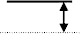
\includegraphics[width=1cm]{./images/bode-approx-konst.png}} &
		\, Konstant: $20 \log \alpha$ &
		\parbox[c][1cm]{1cm}{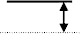
\includegraphics[width=1cm]{./images/bode-approx-konst.png}} &
		Konstant: $\beta$
		\\ \hline
		Pol im Ursprung &
		$\frac{\alpha}{s}$ &
		\parbox[c][1cm]{1cm}{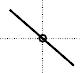
\includegraphics[width=1cm]{./images/bode-approx-ampl-tp-ord1.png}} & 
		\begin{tabular}{l}
			Lineare Steigung: $-20 dB/Dek.$ \\
			$0dB$ bei $\omega = \alpha$
		\end{tabular} &
		\parbox[c][1cm]{1cm}{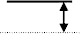
\includegraphics[width=1cm]{./images/bode-approx-konst.png}} & 
		Konstant: $-\frac{\pi}{2}$ 
		\\ \hline
		Nullstelle im Ursprung &
		$\alpha s$ &
		\parbox[c][1cm]{1cm}{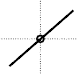
\includegraphics[width=1cm]{./images/bode-approx-ampl-hp-ord1.png}} & 
		\begin{tabular}{l}
			Lineare Steigung: $+20 dB/Dek.$ \\
			$0dB$ bei $\omega = \frac{1}{\alpha}$
		\end{tabular} &
		\parbox[c][1cm]{1cm}{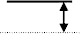
\includegraphics[width=1cm]{./images/bode-approx-konst.png}} &
		Konstant: $+\frac{\pi}{2}$
		\\ \hline	
		Reeller Pol (TP 1.Ord) &
		$\frac{1}{s + \alpha}$ &
		\parbox[c][1cm]{1cm}{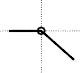
\includegraphics[width=1cm]{./images/bode-approx-ampl-4.png}} &
		\begin{tabular}{ll}
			$\omega < \alpha$: & Konstant $-20 \log \alpha$  \\
			$\omega > \alpha$: & $-20dB/Dek.$
		\end{tabular} &
		\parbox[c][1cm]{1cm}{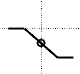
\includegraphics[width=1cm]{./images/bode-approx-phase-4.png}} &
		\begin{tabular}{ll}
			$\omega < \frac{\alpha}{10} $:	& Konstant $0$ \\
			$\omega > 10 \alpha$:		& Konstant $-\frac{\pi}{2}$
		\end{tabular}
		\\ \hline
		Reeller Pol (TP 1.Ord) &
		$\frac{\alpha}{s + \alpha}$ &
		\parbox[c][1cm]{1cm}{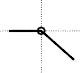
\includegraphics[width=1cm]{./images/bode-approx-ampl-4.png}} &
		\begin{tabular}{ll}
			$\omega < \alpha$: & Konstant $0dB$ \\
			$\omega > \alpha$: & $-20dB/Dek. \qquad (\omega_r = \alpha)$
		\end{tabular} &
		\parbox[c][1cm]{1cm}{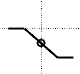
\includegraphics[width=1cm]{./images/bode-approx-phase-4.png}}	& 
		\begin{tabular}{ll}
			$\omega < \frac{\alpha}{10}$: & Konstant $0$ \\
			$\omega > 10 \alpha$: & Konstant $-\frac{\pi}{2}$
		\end{tabular}
		\\ \hline
		Reelle Nullstelle (HP 1.Ord) &
		$s + \alpha$ & 
		\parbox[c][1cm]{1cm}{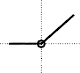
\includegraphics[width=1cm]{./images/bode-approx-ampl-5.png}} &
		\begin{tabular}{ll}
			$\omega < \alpha$: & Konstant $20 \log \alpha$ \\
			$\omega > \alpha$: & $+20dB/Dek.$
		\end{tabular} & 
		\parbox[c][1cm]{1cm}{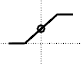
\includegraphics[width=1cm]{./images/bode-approx-phase-5.png}}	&
		\begin{tabular}{ll}
			$\omega < \frac{\alpha}{10}$: & Konstant $0$ \\
			$\omega > 10 \alpha$: & Konstant $+\frac{\pi}{2}$
		\end{tabular}
		\\ \hline	
		Reelle Nullstelle (HP 1.Ord) &
		$\frac{s + \alpha}{\alpha}$ &
		\parbox[c][1cm]{1cm}{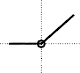
\includegraphics[width=1cm]{./images/bode-approx-ampl-5.png}} &
		\begin{tabular}{ll}
			$\omega < \alpha$: & Konstant $0dB$ \\
			$\omega > \alpha$: & $+20dB/Dek.$
		\end{tabular} &
		\parbox[c][1cm]{1cm}{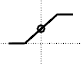
\includegraphics[width=1cm]{./images/bode-approx-phase-5.png}} &
		\begin{tabular}{ll}
			$\omega < \frac{\alpha}{10}$: & Konstant $0$ \\
			$\omega > 10 \alpha$: & Konstant $+\frac{\pi}{2}$
		\end{tabular}
		\\ \hline
		Konjugiert-komplexe Pole \newline
		für $|q_p| > 1/2$ (TP 2.Ord) &
		$\frac{1}{s^2+s\frac{\omega_p}{q_p}+\omega_p^2}$ &
		\parbox[c][1cm]{1cm}{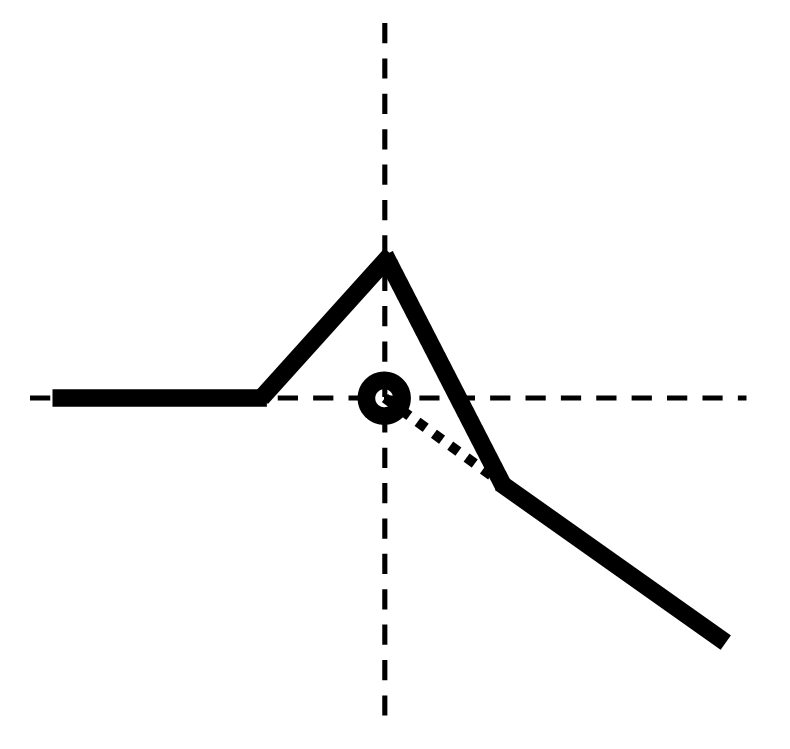
\includegraphics[width=1cm]{./images/bode-approx-ampl-6.png}} &
		\begin{tabular}{ll}
			$\omega < \omega_p$: 	& Konstant $-40 \log \omega_p$ \\
			$\omega > \omega_p$:	& $-40dB/Dek.$ \\
			Überhöhung: 			& $\frac{\omega_p}{2}$ bis $2\omega_p$ \\
			Maximum:				& $-40\log\omega_p + 20 \log q_p$ bei $\omega = \omega_p$			
		\end{tabular} &
		\parbox[c][1cm]{1cm}{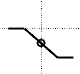
\includegraphics[width=1cm]{./images/bode-approx-phase-6.png}} &
		\begin{tabular}{ll}
			$\omega < \frac{\omega_p}{10^{\frac{1}{2q_p}}}$:	& Konstant $0$ \\
			$\omega > \omega_p 10^{\frac{1}{2q_p}}$:			& Konstant $-\pi$ \\
			$\omega = \omega_p$:								& $-\frac{\pi}{2}$
		\end{tabular}
		\\ \hline
		Konjugiert-komplexe Pole \newline
		für $|q_p| > 1/2$ (TP 2.Ord)&
		$\frac{\omega_p^2}{s^2+s\frac{\omega_p}{q_p}+\omega_p^2}$ & 
		\parbox[c][1cm]{1cm}{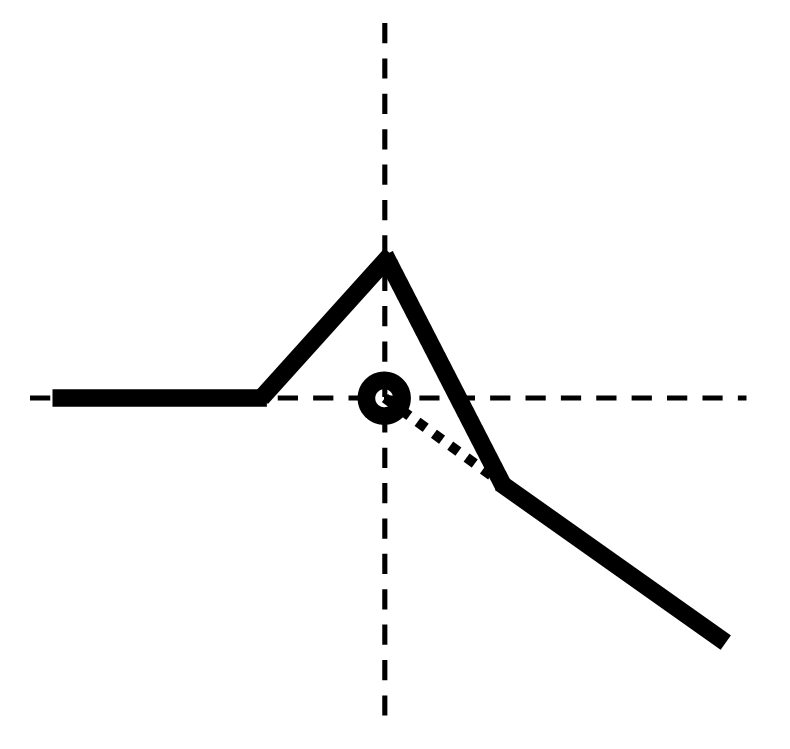
\includegraphics[width=1cm]{./images/bode-approx-ampl-6.png}} &
		\begin{tabular}{ll}
			$\omega < \omega_p$:	& Konstant $0dB$ \\
			$\omega > \omega_p$:	& $-40dB/Dek.$ \\
			Überhöhung:				& $\frac{\omega_p}{2}$ bis $2 \omega_p$ \\
			Maximum:				& $20 \log q_p$ bei $\omega = \omega_p$
		\end{tabular} &
		\parbox[c][1cm]{1cm}{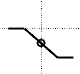
\includegraphics[width=1cm]{./images/bode-approx-phase-6.png}}	& 
		\begin{tabular}{ll}
			$\omega < \frac{\omega_p}{10^{\frac{1}{2q_p}}}$:	& Konstant $0$ \\
			$\omega > \omega_p 10^{\frac{1}{2q_p}}$:			& Konstant $-\pi$ \\
			$\omega = \omega_p$:								& $-\frac{\pi}{2}$
		\end{tabular}
		\\ \hline	
		Konjugiert-komplexe Nullstellen
		für $|q_z| > 1/2$ (HP 2.Ord)&
		$s^2+s\frac{\omega_z}{q_z}+\omega_z^2$ &
		\multicolumn{4}{l|}{
			Analog zu den Konjugiert-komplexen Polen jedoch gespiegelt an der $0dB$- / $0$-Grad-Linie.
		}
		\\
		&
		$\frac{s^2+s\frac{\omega_z}{q_z}+\omega_z^2}{\omega_z^2}$ &
		\multicolumn{4}{l|}{}
		\\ \hline
		\multicolumn{6}{|p{21cm}|}{
			Serieschaltung von Systemen erfolgt durch \textbf{Superposition} der einzelnen Bode-Diagramme 
			(Multiplikation von UTFs entspricht Addition im	dB-Bereich). $\alpha , \beta \in \mathbf{R}$. 
			Für $\omega_p$ und $q_p$ siehe Kapitel\ref{frequenzgang}
		}
		\\ \hline
	\end{longtable}
	\renewcommand{\arraystretch}{\arraystretchOriginal}
\end{landscape}
\clearpage

\subsection{Grundglieder}
Weitere Grundglieder auf \script{202}
\begin{longtable}{|c|c|l|}
	\specialrule{2pt}{0pt}{0pt}
	{\bf Typ} & {\it Symbol} & {\it Gleichung, DGL}\\
	& & {\it Sprungantwort}\\
	& & {\it Frequenzgang, Betrag und Argument}\\ \cline{2-3}
	& Strukturbild & {\it Nyquistdiagramm} -- {\it Bodediagramm}\\
	\specialrule{2pt}{0pt}{0pt}
	
	
	%P-Glied
	P & \parbox[c][2cm]{3cm}{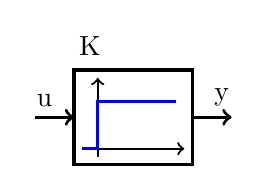
\begin{tikzpicture}
  \begin{scope}[very thick]
    \draw[->] (0,0) -- +(0.5,0) node[near start, above] {u};
    \draw (0.5,-0.6) rectangle +(1.5,1.2);
    \draw[->] (2,0) -- +(0.5,0) node[near end, above] {y};
  \end{scope}

  \node at (0.7,0.9) {K};

  % Inhalt
  \begin{scope}[shift={(0.8,-0.4)}]
    \draw[->, thick] (-0.2,0) -- +(1.3,0);
    \draw[->, thick] (0,-0.1) -- +(0,1);

    \draw[blue, very thick] (-0.2,0) -- ++(0.2,0)
       -- ++(0,0.6) -- +(1,0);
  \end{scope}
\end{tikzpicture}}
	&
	\begin{tabular}{lll}
		$y = Ku$ 		& 							& \\
		$u=1(t)$ 		& $y=K 1(t)$ 				& \\
		$G(j \omega)=K$	& $\left| G \right| = K$	& $arg(G)=0$ \\
	\end{tabular} 
	\\ \cline{2-3}
	& \parbox[c][2cm]{3cm}{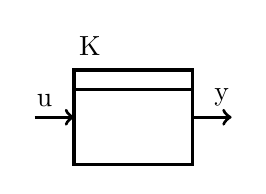
\begin{tikzpicture}
  % Box
  \begin{scope}[very thick]
    \draw[->] (0,0) -- +(0.5,0) node[near start, above] {u};
    \draw (0.5,-0.6) rectangle +(1.5,1.2);
    \draw[->] (2,0) -- +(0.5,0) node[near end, above] {y};
  \end{scope}

  % Zugemüse
  \node at (0.7,0.9) {K};
  \draw[very thick] (0.5, 0.35) -- +(1.5,0);
\end{tikzpicture}}
	& 
	\parbox[c]{3cm}{\usepgflibrary{shapes.misc}
\begin{tikzpicture}
\draw[->, thick] (-0.5,0) -- (2,0) node[below] {Re};
\draw[->, thick] (0,-0.3) -- (0,1) node[left] {Im};
\node[rounded rectangle, draw=blue, thick]  at (1,0) {};
\node at (1,0.4) {K};
\node at (0.8,-0.8) {\small{frequenzunabhängig}};
\end{tikzpicture}} \quad
	\parbox[c]{6cm}{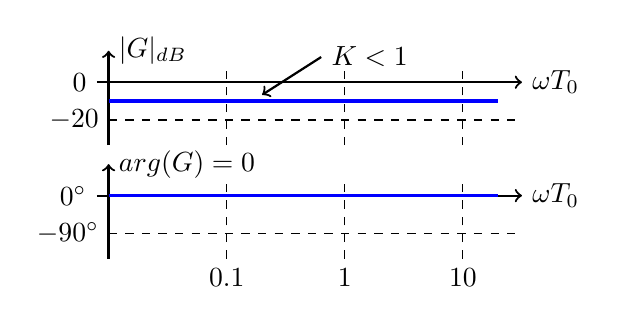
\begin{tikzpicture}[xscale=1.5, yscale=0.8]

%% Amplitude
\begin{scope}
	%% Koordinatensystem
	\draw[thick, ->] (-0.1,0) node[left] {$0$} -- (3.5,0) node[right] {$\omega T_0$};
	\draw[thick, ->] (0,-1) -- (0,0.5) node[right] {$|G|_{dB}$};
	\draw[dashed] (0,-0.6) node[left] {$-20$} -- (3.5,-0.6);
	\draw[dashed] (1,-1) -- +(0,1.2);
	\draw[dashed] (2,-1) -- +(0,1.2);
	\draw[dashed] (3,-1) -- +(0,1.2);
	%%%%%%%%%%%%%%%%

	%% Amplitudengang
	\draw[blue, very thick] (0,-0.3) -- +(3.3,0);
	\draw[<-, thick] (1.3,-0.2) -- +(0.5,0.6) node[right] {$K<1$};
\end{scope}


%% Phase
\begin{scope}[shift={(0,-1.8)}]
	%% Koordinatensystem
	\draw[thick, ->] (-0.1,0) node[left] {$0^\circ$} -- (3.5,0) node[right] {$\omega T_0$};
	\draw[thick, ->] (0,-1) -- (0,0.5) node[right] {$arg(G)=0$};
	\draw[dashed] (0,-0.6) node[left] {$-90^\circ$} -- (3.5,-0.6);
	\draw[dashed] (1,-1) node[below] {$0.1$} -- +(0,1.2);
	\draw[dashed] (2,-1) node[below] {$1$} -- +(0,1.2);
	\draw[dashed] (3,-1) node[below] {$10$} -- +(0,1.2);
	%%%%%%%%%%%%%%%%

	%% Amplitudengang
	\draw[blue, very thick] (0,0) -- +(3.3,0);
\end{scope}

%\draw (current bounding box.south west) rectangle (current bounding box.north east);

\end{tikzpicture}}			 
	\\
	\specialrule{2pt}{0pt}{0pt}
	
	
	%I-Glied
	I & \parbox[c][2cm]{3cm}{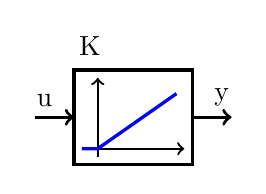
\begin{tikzpicture}
  \begin{scope}[very thick]
    \draw[->] (0,0) -- +(0.5,0) node[near start, above] {u};
    \draw (0.5,-0.6) rectangle +(1.5,1.2);
    \draw[->] (2,0) -- +(0.5,0) node[near end, above] {y};
  \end{scope}

  \node at (0.7,0.9) {K};

  % Inhalt
  \begin{scope}[shift={(0.8,-0.4)}]
    \draw[->, thick] (-0.2,0) -- +(1.3,0);
    \draw[->, thick] (0,-0.1) -- +(0,1);

    \draw[blue, very thick] (-0.2,0) -- ++(0.2,0) -- +(1,0.7);
  \end{scope}

\end{tikzpicture}}
	&
	\begin{tabular}{lll}
		$\dot{y} = Ku$ 					
		& \multicolumn{2}{l}{$y = K \int\limits_{0}^{t}u(\tau)\;d\tau \qquad y(0) = 0 \qquad [K] = sec^{-1}$}										\\
		$u=1(t)$ 						& $y=K t$ 								& \\
		$G(j \omega)=\frac{K}{j\omega}$ & $\left| G \right| = \frac{K}{\omega}$ & $arg(G)=-\frac{\pi}{2}$ \\
	\end{tabular}
	\\ \cline{2-3}
	& \parbox[c][2cm]{3cm}{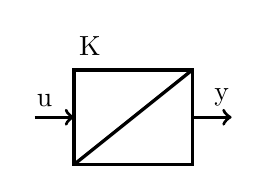
\begin{tikzpicture}
  % Box
  \begin{scope}[very thick]
    \draw[->] (0,0) -- +(0.5,0) node[near start, above] {u};
    \draw (0.5,-0.6) rectangle +(1.5,1.2);
    \draw[->] (2,0) -- +(0.5,0) node[near end, above] {y};
  \end{scope}

  % Zugemüse
  \node at (0.7,0.9) {K};
  \draw[very thick] (0.5, -0.6) -- +(1.5,1.2);
\end{tikzpicture}}
	&
	\parbox[c]{3cm}{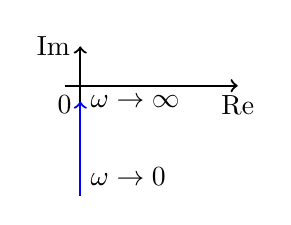
\begin{tikzpicture}
\draw[->, thick] (-0.2,0) node[below] {0} -- (2,0) node[below] {Re};
\draw[->, thick] (0,-1) -- (0,0.5) node[left] {Im};

\draw[->, blue, thick] (0,-1.4) node[above right, black] {$\omega \rightarrow 0$} 
	-- (0,-0.2) node[right, black] {$\omega \rightarrow \infty$};
%\draw (current bounding box.south west) rectangle (current bounding box.north east);
\end{tikzpicture}}
	\parbox[c]{6cm}{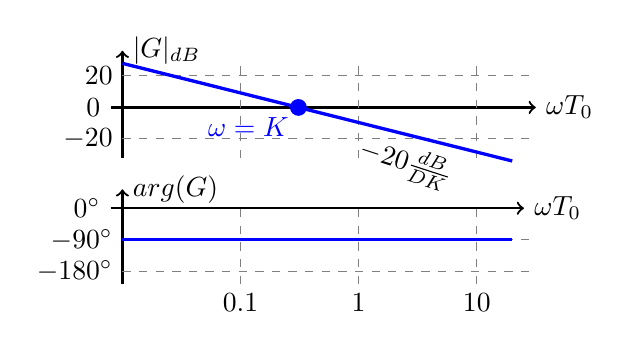
\begin{tikzpicture}[xscale=1.5, yscale=0.8]
	%% Amplitude
\begin{scope}
	%% Koordinatensystem
	\draw[thick, ->] (0,-1.2) -- (0,0.5) node[right] {$|G|_{dB}$};
	\draw[thick, ->] (-0.1,-0.4) node[left] {$0$} -- +(3.6,0) node[right] {$\omega T_0$};
	\draw[dashed,gray] (0,-0.9) node[left, black] {$-20$} -- +(3.5,0);
	\draw[dashed,gray] (0,0.1) node[left, black] {$20$} -- +(3.5,0);
	\draw[dashed,gray] (1,-1.2) -- +(0,1.5);
	\draw[dashed,gray] (2,-1.2) -- +(0,1.5);
	\draw[dashed,gray] (3,-1.2) -- +(0,1.5);
	%%%%%%%%%%%%%%%%

	%% Amplitudengang
	\draw[blue, very thick] (0,0.3) -- +(3.3,-1.55) node[near end, below, rotate=-18, black] {$-20\frac{dB}{DK}$};
	\draw(1.49,-0.4) node[draw,circle,inner sep=2pt,fill, blue] {};
	\node at (1.49, -0.4) [anchor = north east, blue] {$\omega = K$};
	
\end{scope}


%% Phase
\begin{scope}[shift={(0,-2.2)}]
	%% Koordinatensystem
	\draw[thick, ->] (-0.1,0.2) node[left] {$0^\circ$} -- +(3.5,0) node[right] {$\omega T_0$};
	\draw[thick, ->] (0,-1) -- (0,0.5) node[right] {$arg(G)$};
	\draw[dashed,gray] (0,-0.3) node[left, black] {$-90^\circ$} -- +(3.5,0);
	\draw[dashed,gray] (0,-0.8) node[left, black] {$-180^\circ$} -- +(3.5,0);
	\draw[dashed, gray] (1,-1) node[below, black] {$0.1$} -- +(0,1.2);
	\draw[dashed,gray] (2,-1) node[below, black] {$1$} -- +(0,1.2);
	\draw[dashed,gray] (3,-1) node[below, black] {$10$} -- +(0,1.2);
	%%%%%%%%%%%%%%%%

	%% Amplitudengang
	\draw[blue, very thick] (0,-0.3) -- +(3.3,0);
\end{scope}

%\draw (current bounding box.south west) rectangle (current bounding box.north east);
\end{tikzpicture}} 
	\\
	\specialrule{2pt}{0pt}{0pt}
	
	
	%D-Glied
	D & \parbox[c][2cm]{3cm}{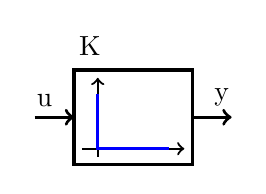
\begin{tikzpicture}
  \begin{scope}[very thick]
    \draw[->] (0,0) -- +(0.5,0) node[near start, above] {u};
    \draw (0.5,-0.6) rectangle +(1.5,1.2);
    \draw[->] (2,0) -- +(0.5,0) node[near end, above] {y};
  \end{scope}

  \node at (0.7,0.9) {K};

  % Inhalt
  \begin{scope}[shift={(0.8,-0.4)}]
    \draw[->, thick] (-0.2,0) -- +(1.3,0);
    \draw[->, thick] (0,-0.1) -- +(0,1);

    \draw[blue, very thick] (0,0.7) -- ++(0,-0.7) -- +(0.9,0);
  \end{scope}

\end{tikzpicture}}
	&
	\begin{tabular}{lll}
		$y = K\dot{u}$					
		&	$[K] =sec$					& \\
		$u=1(t)$						& $y=K \delta (t)$						& \\
		$G(j \omega)=K j\omega$			& $\left| G \right| = K\omega$			& $arg(G)=\frac{\pi}{2}$
	\end{tabular}
	\\ \cline{2-3}
	& \parbox[c][2cm]{3cm}{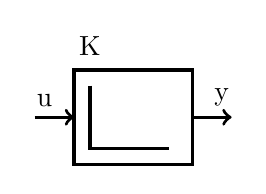
\begin{tikzpicture}
  % Box
  \begin{scope}[very thick]
    \draw[->] (0,0) -- +(0.5,0) node[near start, above] {u};
    \draw (0.5,-0.6) rectangle +(1.5,1.2);
    \draw[->] (2,0) -- +(0.5,0) node[near end, above] {y};
  \end{scope}

  % Zugemüse
  \node at (0.7,0.9) {K};
  \draw[very thick] (0.7, 0.4) -- ++(0,-0.8) -- ++(1,0);
\end{tikzpicture}}			
	&
	\parbox[c]{3cm}{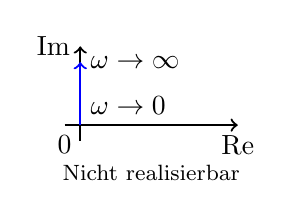
\begin{tikzpicture}
\draw[->, thick] (-0.2,0) node[below] {0} -- (2,0) node[below] {Re};
\draw[->, thick] (0,-0.2) -- (0,1) node[left] {Im};

\draw[->, blue, thick] (0,0) node[above right, black] {$\omega \rightarrow 0$} 
	-- (0,0.8) node[right, black] {$\omega \rightarrow \infty$};
\draw[] (0.9,-0.6) node {\footnotesize{Nicht realisierbar}};
%\draw (current bounding box.south west) rectangle (current bounding box.north east);
\end{tikzpicture}}
	\parbox[c]{6cm}{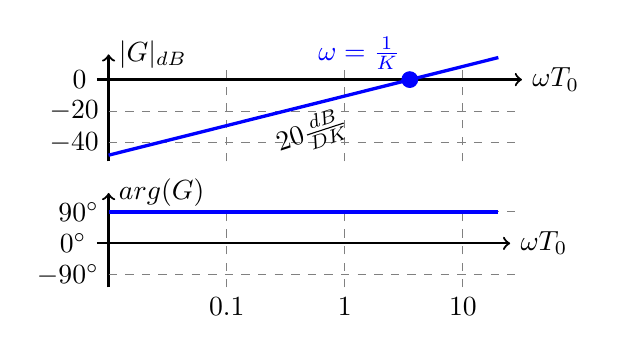
\begin{tikzpicture}[xscale=1.5, yscale=0.8]
	%% Amplitude
\begin{scope}
	%% Koordinatensystem
	\draw[thick, ->] (0,-1.2) -- (0,0.5) node[right] {$|G|_{dB}$};
	\draw[thick, ->] (-0.1,0.1) node[left] {$0$} -- +(3.6,0) node[right] {$\omega T_0$};
	\draw[dashed,gray] (0,-0.9) node[left, black] {$-40$} -- +(3.5,0);
	\draw[dashed,gray] (0,-0.4) node[left, black] {$-20$} -- +(3.5,0);
	\draw[dashed,gray] (1,-1.2) -- +(0,1.5);
	\draw[dashed,gray] (2,-1.2) -- +(0,1.5);
	\draw[dashed,gray] (3,-1.2) -- +(0,1.5);
	%%%%%%%%%%%%%%%%

	%% Amplitudengang
	\draw[blue, very thick] (0,-1.1) -- +(3.3,1.55) node[midway, below, rotate=18, black] {$20\frac{dB}{DK}$};
	\draw(2.55,0.1) node[draw,circle,inner sep=2pt,fill, blue] {};
	\node at (2.55, 0.1) [anchor = south east, blue] {$\omega = \frac{1}{K}$};
\end{scope}


%% Phase
\begin{scope}[shift={(0,-2.2)}]
	%% Koordinatensystem
	\draw[thick, ->] (-0.1,-0.3) node[left] {$0^\circ$} -- +(3.5,0) node[right] {$\omega T_0$};
	\draw[thick, ->] (0,-1) -- (0,0.5) node[right] {$arg(G)$};
	\draw[dashed,gray] (0,0.2) node[left, black] {$90^\circ$} -- +(3.5,0);
	\draw[dashed,gray] (0,-0.8) node[left, black] {$-90^\circ$} -- +(3.5,0);
	\draw[dashed, gray] (1,-1) node[below, black] {$0.1$} -- +(0,1.2);
	\draw[dashed,gray] (2,-1) node[below, black] {$1$} -- +(0,1.2);
	\draw[dashed,gray] (3,-1) node[below, black] {$10$} -- +(0,1.2);
	%%%%%%%%%%%%%%%%

	%% Amplitudengang
	\draw[blue, very thick] (0,0.2) -- +(3.3,0);
\end{scope}

%\draw (current bounding box.south west) rectangle (current bounding box.north east);
\end{tikzpicture}} 
	\\
	\specialrule{2pt}{0pt}{0pt}
		\newpage
\specialrule{2pt}{0pt}{0pt}
	
	%PT1_Glied
	$PT_1$ & \parbox[c][2cm]{3cm}{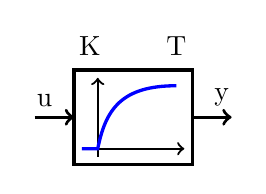
\begin{tikzpicture}
  \begin{scope}[very thick]
    \draw[->] (0,0) -- +(0.5,0) node[near start, above] {u};
    \draw (0.5,-0.6) rectangle +(1.5,1.2);
    \draw[->] (2,0) -- +(0.5,0) node[near end, above] {y};
  \end{scope}

  \node at (0.7,0.9) {K};
  \node at (1.8,0.9) {T};

  % Inhalt
  \begin{scope}[shift={(0.8,-0.4)}]
    \draw[->, thick] (-0.2,0) -- +(1.3,0);
    \draw[->, thick] (0,-0.1) -- +(0,1);

    \draw[blue, very thick] (-0.2,0) -- ++(0.2,0)
              .. controls (0.1,0.5) and (0.3,0.8) .. (1,0.8);
  \end{scope}

\end{tikzpicture}}
	&
	\begin{tabular}{lll}
		$T\dot{y}+y=Ku$							& $y(0)=0$									& \\
		$u=1(t)$								& $y=K \left[ 1-e^{- \frac{t}{T}}\right]$	& \\
		$G(j \omega)= \frac{K}{1+j\omega T}$	& $\left| G \right| = \frac{K}{\sqrt{1+(\omega T)^2}}$ &
		$arg(G)=-\arctan(\omega T)$
	\end{tabular}
	\\ \cline{2-3}
	& \parbox[c][2cm]{3cm}{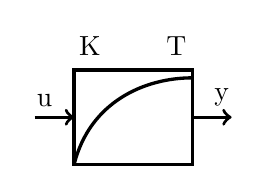
\begin{tikzpicture}
  \begin{scope}[very thick]
    \draw[->] (0,0) -- +(0.5,0) node[near start, above] {u};
    \draw (0.5,-0.6) rectangle +(1.5,1.2);
    \draw[->] (2,0) -- +(0.5,0) node[near end, above] {y};
  \end{scope}

 % Zugemüse
 \node at (0.7,0.9) {K};
 \node at (1.8,0.9) {T};
 \draw[very thick] (0.5,-0.6)  .. controls (0.7,0.2) and (1.4,0.5) .. (2,0.5);

\end{tikzpicture}}	
	&
	\parbox[c]{3.7cm}{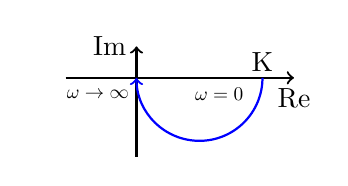
\begin{tikzpicture}
\draw[->, thick] (-0.9,0) -- (2,0) node[below] {Re};
\draw[->, thick] (0,-1) -- (0,0.4) node[left] {Im};

\node at (1.6,0.2) {K};
\draw[blue, thick, ->] (1.6,0) arc (0:-180:0.8);

\scalebox{0.7}{
  \node at (-0.7,-0.3) {$\omega \rightarrow \infty$};
  \node at (1.5, -0.3) {$\omega = 0$};
}
\end{tikzpicture}}
	\parbox[c]{6cm}{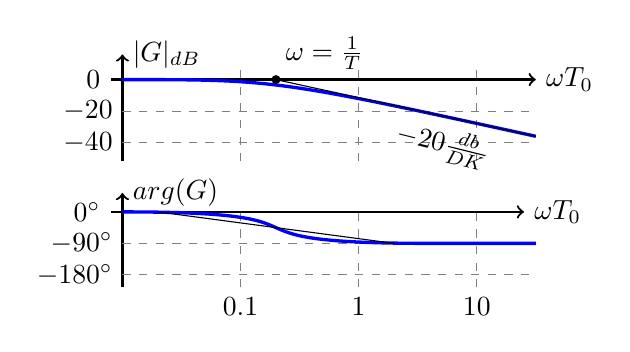
\begin{tikzpicture}[xscale=1.5, yscale=0.8]
	%% Amplitude
\begin{scope}
	%% Koordinatensystem
	\draw[thick, ->] (0,-1.2) -- (0,0.5) node[right] {$|G|_{dB}$};
	\draw[dashed,gray] (1,-1.2) -- +(0,1.5);
	\draw[dashed,gray] (2,-1.2) -- +(0,1.5);
	\draw[dashed,gray] (3,-1.2) -- +(0,1.5);
	
	\draw[thick, ->] (-0.1,0.1) node[left] {$0$} -- +(3.6,0) node[right] {$\omega T_0$};
	\draw[dashed,gray] (0,-0.9) node[left, black] {$-40$} -- +(3.5,0);
	\draw[dashed,gray] (0,-0.4) node[left, black] {$-20$} -- +(3.5,0);

	%%%%%%%%%%%%%%%%

	%% Amplitudengang
	\draw[blue, very thick] (0,0.1) .. controls (1.3,0.1) .. (3.5,-0.8) 
	node[very near end, below, rotate=-14, color=black] {$-20 \frac{db}{DK}$};
	\draw (1.3,0.1) -- (3.5, -0.8);
	\draw(1.3,0.1) node[draw,circle,inner sep=1pt,fill] {};
	\node at (1.3, 0.1) [anchor = south west] {$\omega = \frac{1}{T}$};
\end{scope}


%% Phase
\begin{scope}[shift={(0,-2.2)}]
	%% Koordinatensystem
	\draw[thick, ->] (0,-1) -- (0,0.5) node[right] {$arg(G)$};
	\draw[dashed, gray] (1,-1) node[below, black] {$0.1$} -- +(0,1.2);
	\draw[dashed,gray] (2,-1) node[below, black] {$1$} -- +(0,1.2);
	\draw[dashed,gray] (3,-1) node[below, black] {$10$} -- +(0,1.2);
	
	\draw[thick, ->] (-0.1,0.2) node[left] {$0^\circ$} -- +(3.5,0) node[right] {$\omega T_0$};
	\draw[dashed,gray] (0,-0.3) node[left, black] {$-90^\circ$} -- +(3.5,0);
	\draw[dashed,gray] (0,-0.8) node[left, black] {$-180^\circ$} -- +(3.5,0);

	%%%%%%%%%%%%%%%%

	%% Amplitudengang
	\draw[blue, very thick] (0,0.2) .. controls (2.0,0.2) and (0.6,-0.3) .. (2.6,-0.3) -- +(0.9,0);
	\draw (0.3,0.2) -- (2.3,-0.3);
	
\end{scope}

%\draw (current bounding box.south west) rectangle (current bounding box.north east);
\end{tikzpicture}}
	\\
	\specialrule{2pt}{0pt}{0pt}
	

	
	%PT2_Glied
	$PT_2$ &
	\begin{minipage}{3cm}
		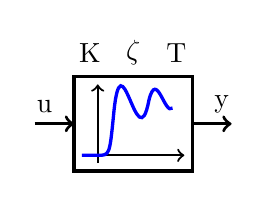
\begin{tikzpicture}
  \begin{scope}[very thick]
    \draw[->] (0,0) -- +(0.5,0) node[near start, above] {u};
    \draw (0.5,-0.6) rectangle +(1.5,1.2);
    \draw[->] (2,0) -- +(0.5,0) node[near end, above] {y};
  \end{scope}

  \node at (0.7,0.9) {K};
  \node at (1.25,0.9) {$\zeta$};
  \node at (1.8,0.9) {T};

  % Inhalt
  \begin{scope}[shift={(0.8,-0.4)}]
    \draw[->, thick] (-0.2,0) -- +(1.3,0);
    \draw[->, thick] (0,-0.1) -- +(0,1);

	\draw[blue, very thick] (-0.2,0) -- ++(0.2,0)
              .. controls (0.15,0) .. (0.2,0.5)
              .. controls (0.3,1.6)  and (0.5,-0.1) .. (0.65,0.7)
              .. controls (0.75,1.1)  and (0.85,0.5) .. (0.95,0.6)
              ;
  \end{scope}
\end{tikzpicture}
	\end{minipage}
	&
	\begin{tabular}{lll}
		$T^2\ddot{y}+2\zeta T \dot{y}+y=Ku$ & $\ddot{y}+2\zeta\omega_n \dot{y}+\omega_n^2y=K\omega_n^2u$ & \\
		$y(0)=0$ & $\dot{y}(0)=0$ & $\omega_n=\frac{1}{T}$ \\
		\multicolumn{3}{l}{
			$y=K \left[1-\frac{1}{\sqrt{1-\zeta^2}}e^{-\zeta\omega_n t}\sin
			\left( \sqrt{1-\zeta^2} \omega_n t+arcos(\zeta) \right)\right]$
		} \\
		$G(j \omega)= \frac{K}{1+ 2 \zeta (j\omega) T  + (j \omega T)^2}$ & $\left| G \right| = \frac{K}{\sqrt{\left[1+(j\omega
				T)^2\right]^2+\left[2\zeta \omega T \right]^2}}$ & \\
		$\arg(G)=-\arctan  \frac{2\zeta \omega T}{1+(j\omega T)^2}$ & $0 \leq\omega T \leq 1$ & \\
		$\arg(G)=\arctan \frac{2\zeta \omega T}{1+(j \omega T)^2}-\pi$ & $1 \leq\omega T \leq \infty$ & \\
		
	\end{tabular}
	\\ \cline{2-3}
	& \parbox[c][2cm]{3cm}{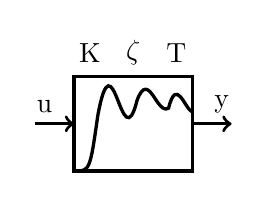
\begin{tikzpicture}
  \begin{scope}[very thick]
    \draw[->] (0,0) -- +(0.5,0) node[near start, above] {u};
    \draw (0.5,-0.6) rectangle +(1.5,1.2);
    \draw[->] (2,0) -- +(0.5,0) node[near end, above] {y};
  \end{scope}

   \node at (0.7,0.9) {K};
    \node at (1.25,0.9) {$\zeta$};
    \node at (1.8,0.9) {T};

  % Inhalt
  \begin{scope}[shift={(0.8,-0.4)}]

	\draw[very thick] (-0.3,-0.2)
              .. controls (-0.1,-0.2) .. (0.0,0.5)
              .. controls (0.2,1.6)  and (0.3,-0.1) .. (0.5,0.7)
              .. controls (0.65,1.1)  and (0.75,0.5) .. (0.9,0.6)
              .. controls (1.0,1.0) and (1.1, 0.6) ..
              (1.2, 0.55)
              ;
  \end{scope}
\end{tikzpicture}}
	& \begin{minipage}{4cm}
		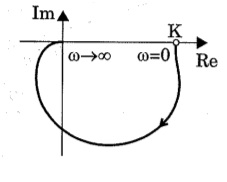
\includegraphics[angle = {-0.3}, width=4cm]{./images/PT2_Nyq.jpg}
	\end{minipage}
	\begin{minipage}{8cm}
		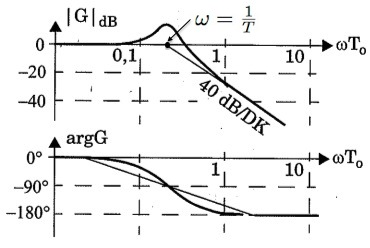
\includegraphics[angle = {0.2}, width=7cm]{./images/PT2_Bode.jpg}
	\end{minipage} \rule[-5mm]{0mm}{35mm}
	\\
	\specialrule{2pt}{0pt}{0pt}
	
	
	%Tt_Glied
	$T_t$ &
	\parbox[c][2cm]{3cm}{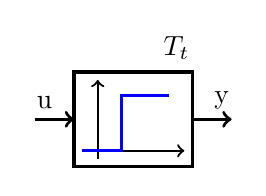
\begin{tikzpicture}
  \begin{scope}[very thick]
    \draw[->] (0,0) -- +(0.5,0) node[near start, above] {u};
    \draw (0.5,-0.6) rectangle +(1.5,1.2);
    \draw[->] (2,0) -- +(0.5,0) node[near end, above] {y};
  \end{scope}

  \node at (1.8,0.9) {$T_t$};

  % Inhalt
  \begin{scope}[shift={(0.8,-0.4)}]
    \draw[->, thick] (-0.2,0) -- +(1.3,0);
    \draw[->, thick] (0,-0.1) -- +(0,1);

    \draw[blue, very thick] (-0.2,0) -- ++(0.5,0) -- ++(0,0.7) -- +(0.6,0);
  \end{scope}

\end{tikzpicture}}
	&
	\begin{tabular}{lll}
		$y=\begin{cases}
			0 & 0<t<T_t \\
			u(t-T_t) & t \geq T_t
		\end{cases}$ & & \\
		$u=1(t)$ & $y=1(t-T_t)$ & \\
		$G(j \omega)= e^{-j\omega T_t}$ & $\left| G \right| = 1$ & $arg(G)=-\omega T_t$
	\end{tabular}
	\\ \cline{2-3}
	& \parbox[c][2cm]{3cm}{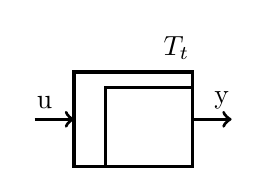
\begin{tikzpicture}
  \begin{scope}[very thick]
    \draw[->] (0,0) -- +(0.5,0) node[near start, above] {u};
    \draw (0.5,-0.6) rectangle +(1.5,1.2);
    \draw[->] (2,0) -- +(0.5,0) node[near end, above] {y};
  \end{scope}

% Zugemüse
\node at (1.8,0.9) {$T_t$};

\draw[very thick] (0.9,-0.6) -- ++(0,1) -- +(1.1,0);
\end{tikzpicture}}
	& 
	\parbox[c]{3cm}{\usetikzlibrary{decorations.markings}
\begin{tikzpicture}
\useasboundingbox (-1.4,-1.4) rectangle (1.9,1.4);
\draw[->, thick] (-1.1,0) -- (1.6,0) node[above] {Re};
\draw[->, thick] (0,-1) -- (0,1.1) node[left] {Im};

\draw (0.8,0.05) arc(90:450:0.05) node[above right] {\small{1}};
\draw (-0.8,0.05) arc(90:450:0.05) node[above left] {\small{-1}};

\draw[blue, thick,
	decoration={
		markings,
		mark= at position 0.9 with {\arrow{<}}
	},
	postaction={decorate}
] (0.8,0) arc (0:360:0.8);

\scalebox{0.7}{
  \node at (1.3,-1.5) {$2\pi$-periodisch};
  \node at (1.6, -0.3) {$\omega = 0$};
}
%\draw (current bounding box.south west) rectangle (current bounding box.north east);
\end{tikzpicture}}
	\parbox[c]{6cm}{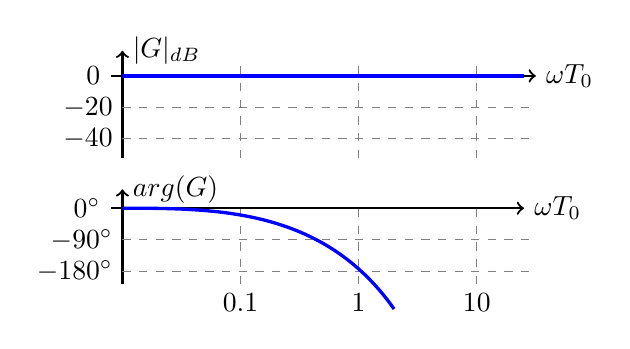
\begin{tikzpicture}[xscale=1.5, yscale=0.8]
	%% Amplitude
\begin{scope}
	%% Koordinatensystem
	\draw[thick, ->] (0,-1.2) -- (0,0.5) node[right] {$|G|_{dB}$};
	\draw[dashed,gray] (1,-1.2) -- +(0,1.5);
	\draw[dashed,gray] (2,-1.2) -- +(0,1.5);
	\draw[dashed,gray] (3,-1.2) -- +(0,1.5);
	
	\draw[thick, ->] (-0.1,0.1) node[left] {$0$} -- +(3.6,0) node[right] {$\omega T_0$};
	\draw[dashed,gray] (0,-0.9) node[left, black] {$-40$} -- +(3.5,0);
	\draw[dashed,gray] (0,-0.4) node[left, black] {$-20$} -- +(3.5,0);

	%%%%%%%%%%%%%%%%

	%% Amplitudengang
	\draw[blue, very thick] (0,0.1) -- +(3.4,0);
\end{scope}


%% Phase
\begin{scope}[shift={(0,-2.2)}]
	%% Koordinatensystem
	\draw[thick, ->] (0,-1) -- (0,0.5) node[right] {$arg(G)$};
	\draw[dashed, gray] (1,-1) node[below, black] {$0.1$} -- +(0,1.2);
	\draw[dashed,gray] (2,-1) node[below, black] {$1$} -- +(0,1.2);
	\draw[dashed,gray] (3,-1) node[below, black] {$10$} -- +(0,1.2);
	
	\draw[thick, ->] (-0.1,0.2) node[left] {$0^\circ$} -- +(3.5,0) node[right] {$\omega T_0$};
	\draw[dashed,gray] (0,-0.3) node[left, black] {$-90^\circ$} -- +(3.5,0);
	\draw[dashed,gray] (0,-0.8) node[left, black] {$-180^\circ$} -- +(3.5,0);

	%%%%%%%%%%%%%%%%

	%% Amplitudengang
	\draw[blue, very thick] (0,0.2) .. controls (0.8,0.2) and (1.7,0.2) .. (2.3,-1.4);	
\end{scope}

%\draw (current bounding box.south west) rectangle (current bounding box.north east);
\end{tikzpicture}}
	\\
	\specialrule{2pt}{0pt}{0pt}
	
	%DT1_Glied
	$DT_1$ &
	\parbox[c][2cm]{3cm}{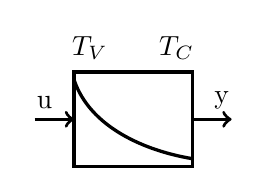
\begin{tikzpicture}
  \begin{scope}[very thick]
    \draw[->] (0,0) -- +(0.5,0) node[near start, above] {u};
    \draw (0.5,-0.6) rectangle +(1.5,1.2);
    \draw[->] (2,0) -- +(0.5,0) node[near end, above] {y};
  \end{scope}

 % Zugem�se
 \node at (0.7,0.9) {$T_V$};
 \node at (1.8,0.9) {$T_C$};
 \draw[very thick] (0.5,0.5)  .. controls (0.7,-0.1) and (1.4,-0.4) .. (2,-0.5);

\end{tikzpicture}}
	&
	\begin{tabular}{lll}
		$G(j \omega)= G_D \cdot G_{PT_1} = j\omega T_V \dfrac{1}{1+j\omega T_C} = \dfrac{T_V}{T_C}\left(1- \dfrac{1}{1+ j\omega T_C} \right)$ \\
	\end{tabular}\\
	\specialrule{2pt}{0pt}{0pt}
\end{longtable}
\clearpage
\twocolumn

\section{Idiotenseite}
\subsection{Differentation}

{\setlength{\extrarowheight}{4pt}
	\begin{tabular}{@{}lcl@{}}
		\textbf{f(x)} & $\rightarrow$ & \textbf{f'(x)} \\
		\toprule
		$c$ & $\rightarrow$ & $0$ \\
		$x^n$  & $\rightarrow$ & $n\cdot x^{n-1}$ \\
		$c\cdot g\left(x\right)$  & $\rightarrow$ & $c\cdot g'\left(x\right)$ \\
		$e^x$  & $\rightarrow$ & $e^x$ \\
		$a^x$ & $\rightarrow$ & $a^x\ln(a)$\\
		\midrule
		$g\left(x\right)+h\left(x\right)$  & $\rightarrow$ & $g'\left(x\right)+h'\left(x\right)$ \\
		$u\left(x\right)\cdot v\left(x\right)$  & $\rightarrow$ & $u'\left(x\right)\cdot v\left(x\right)+u\left(x\right)\cdot v'\left(x\right)$ \\ 
		$\frac{u\left(x\right)}{v\left(x\right)}$  & $\rightarrow$ & $\frac{u'\left(x\right)\cdot v\left(x\right)-u\left(x\right)\cdot v'\left(x\right)}{v^2\left(x\right)}$ \\
		$u\left(v\left(x\right)\right)$  & $\rightarrow$ & $u'\left(v\left(x\right)\right)\cdot v'\left(x\right)$ \\
		\midrule
		$\cos\left(x\right)$ & $\rightarrow$ & $-\sin(x)$ \\
		$\sin\left(x\right)$ & $\rightarrow$ & $\cos(x)$ \\	
		$\cosh\left(x\right)$ & $\rightarrow$ & $\sinh(x)$ \\
		$\sinh\left(x\right)$ & $\rightarrow$ & $\cosh(x)$ \\
		$\tan\left(x\right)$ & $\rightarrow$ & $\frac{1}{\cos^2(x)} = 1 + \tan^2(x)$ \\	
		$\ln\left(x\right)$ & $\rightarrow$ & $\frac{1}{x}$ \\
		$f^{-1}\left(x\right) {\scriptscriptstyle (Umkehrf.)}$  & $\rightarrow$ & $\frac{1}{f'(f^{-1}(x))}$ \\
		$\left|x\right|$ & $\rightarrow$ & $\frac{\left|x\right|}{x}$ \\
	\end{tabular}
}

\subsection{Trigonometire}
\noindent\textbf{Grad zu Bogen}: $ rad = grad \cdot \frac{\pi}{180} $~\\
\noindent\textbf{Bogen zu Grad}: $ grad = rad \cdot \frac{180}{\pi}$
\subsubsection{Einheitskreis}
\begin{center}
	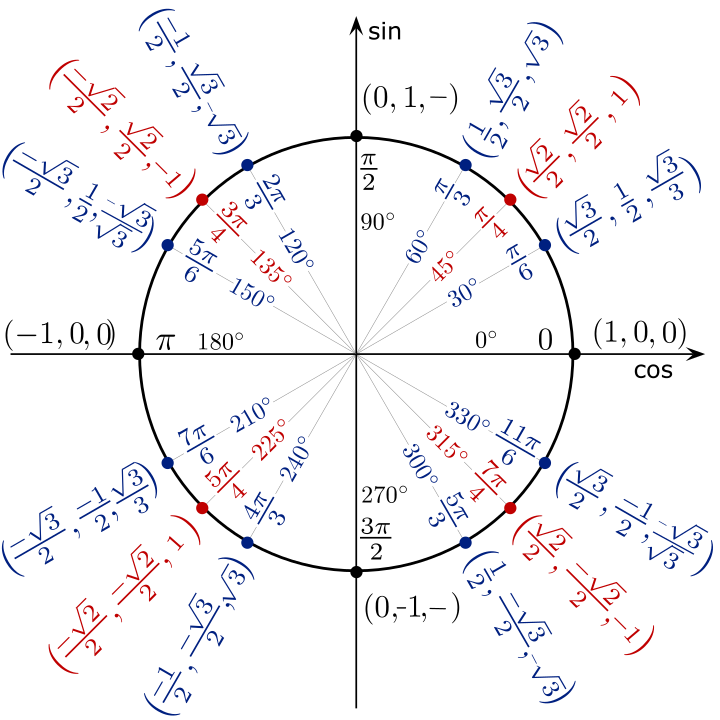
\includegraphics[width=0.8\columnwidth]{Images/einheitskreis}\\
	Punkte auf Kreis [$\cos(\alpha), \sin(\alpha), \tan(\alpha)$]
\end{center}

\subsubsection{Periodizität}
$\cos(a+k\cdot2\pi)=\cos(a) \qquad \sin(a+k\cdot2\pi)=\sin(a) \qquad
(k \in \mathbb{Z})$

\subsubsection{Doppel- und Halbwinkel}	
\begin{align*}
	\sin(2a) &=2\sin(a)\cos(a) &= \frac{2\tan(a)}{1 +\tan^2(a)}\\
	\cos(2a) &=\cos^2(a)-\sin^2(a) &= 2\cos^2(a)-1 &= 1-2\sin^2(a)\\
	\cos^2 \left(\frac{a}{2}\right) &=\frac{1+\cos(a)}{2} \\
	\sin^2 \left(\dfrac{a}{2}\right)&=\frac{1-\cos(a)}{2}
\end{align*}


\subsubsection{Additionstheoreme}
\begin{align*}
	\sin(a \pm b)&=\sin(a) \cdot \cos(b) \pm \cos(a) \cdot \sin(b)\\
	\cos(a \pm b)&=\cos(a) \cdot \cos(b) \mp \sin(a) \cdot \sin(b)\\	
	\tan(a \pm b)&=\dfrac{\tan(a) \pm \tan(b)}{1 \mp \tan(a) \cdot \tan(b)}\\
	\sin(a)+\sin(b) &= 2\sin\left(\frac{a + b}{2}\right)\cos\left(\frac{a - b}{2}\right)\\
	\sin(a)-\sin(b) &= 2\cos\left(\frac{a + b}{2}\right)\sin\left(\frac{a - b}{2}\right)\\
	\cos(a)+\cos(b) &= 2\cos\left(\frac{a + b}{2}\right)\cos\left(\frac{a - b}{2}\right)\\
	\cos(a)-\cos(b) &= -2\sin\left(\frac{a + b}{2}\right)\sin\left(\frac{a - b}{2}\right)\\
	\sin(a)\sin(b)&=\frac{1}{2}(\cos(a-b)-\cos(a+b))\\
	\cos(a)\cos(b)&=\frac{1}{2}(\cos(a-b)+\cos(a+b))\\
	\sin(a)\cos(b)&=\frac{1}{2}(\sin(a-b)+\sin(a+b))\\
\end{align*}

\subsubsection{Potenzen}
\begin{align*}
	\sin^2(a) &= \frac{1}{2}(1 - \cos(2a)) \\
	\sin^3(a) &= \frac{1}{4}(3\sin(a) - \sin(3a)) \\
	\cos^2(a) &= \frac{1}{2}(1 + \cos(2a)) \\
	\cos^3(a) &= \frac{1}{4}(3\cos(a) + \cos(3a)) \\
\end{align*}

\clearpage
\subsection{Log-Tabelle}\label{log_tabelle}
\begin{center}
	\parbox{7cm}{
		\scriptsize
		\begin{tabular}{l|l|l|l}
			\textbf{Lrel. (dB)} & \textbf{Lrel. (NP)} & \textbf{P2/P1} & \textbf{A2/A1} \\ \toprule
			$100.000$ & $11.513$ & $10^{10}$ & $10^5$ \\ \hline
			$90.000$ & $10.362$ & $10^9$ & $31622.777$ \\ \hline
			$80.000$ & $9.210$ & $10^8$ & $10^4$ \\ \hline
			$70.000$ & $8.059$ & $10^7$ & $3162.278$ \\ \hline
			$60.000$ & $6.908$ & $10^6$ & $10^3$ \\ \hline
			$50.000$ & $5.756$ & $10^5$ & $316.228$ \\ \hline
			$40.000$ & $4.605$ & $10^4$ & $10^2$ \\ \hline
			$30.000$ & $3.454$ & $10^3$ & $31.623$ \\ \hline
			\textbf{$20.000$} & $2.303$ & \textbf{$10^2$} & \textbf{$10.000$} \\ \hline
			$19.085$ & $2.197$ & $81.000$ & $9.000$ \\ \hline
			$19.000$ & $2.187$ & $79.433$ & $8.913$ \\ \hline
			$18.062$ & $2.079$ & $64.000$ & $8.000$ \\ \hline
			$18.000$ & $2.072$ & $63.096$ & $7.943$ \\ \hline
			$17.000$ & $1.957$ & $50.119$ & $7.079$ \\ \hline
			$16.902$ & $1.946$ & $49.000$ & $7.000$ \\ \hline
			$16.000$ & $1.842$ & $39.811$ & $6.310$ \\ \hline
			$15.563$ & $1.792$ & $36.000$ & $6.000$ \\ \hline
			$15.000$ & $1.727$ & $31.623$ & $5.623$ \\ \hline
			$14.000$ & $1.612$ & $25.119$ & $5.012$ \\ \hline
			\textbf{$13.979$} & $1.609$ & \textbf{$25.000$} & \textbf{$5.000$} \\ \hline
			$13.000$ & $1.497$ & $19.953$ & $4.467$ \\ \hline
			\textbf{$12.041$} & $1.386$ & \textbf{$16.000$} & \textbf{$4.000$} \\ \hline
			\textbf{$12.000$} & $1.382$ & $15.849$ & $3.981$ \\ \hline
			$11.000$ & $1.266$ & $12.589$ & $3.548$ \\ \hline
			\textbf{$10.000$} & $1.151$ & \textbf{$10.000$} & $3.162$ \\ \hline
			$9.542$ & $1.099$ & $9.000$ & $3.000$ \\ \hline
			$9.000$ & $1.036$ & $7.943$ & $2.818$ \\ \hline
			$8.000$ & $0.921$ & $6.310$ & $2.512$ \\ \hline
			$7.000$ & $0.806$ & $5.012$ & $2.239$ \\ \hline
			\textbf{$6.021$} & \textbf{$0.693$} & \textbf{$4.000$} & \textbf{$2.000$} \\ \hline
			$6.000$ & $0.691$ & $3.981$ & $1.995$ \\ \hline
			$5.000$ & $0.576$ & $3.162$ & $1.778$ \\ \hline
			$4.000$ & $0.461$ & $2.512$ & $1.585$ \\ \hline
			\textbf{$3.010$} & \textbf{$0.347$} & \textbf{$2.000$} & \textbf{$1.414$} \\ \hline
			$3.000$ & $0.345$ & $1.995$ & $1.413$ \\ \hline
			$2.000$ & $0.230$ & $1.585$ & $1.259$ \\ \hline
			$1.000$ & $0.115$ & $1.259$ & $1.122$ \\ \hline
			$0.000$ & $0.000$ & $1.000$ & $1.000$ \\ \hline
			-$1.000$ & -$0.115$ & $0.794$ & $0.891$ \\ \hline
			-$2.000$ & -$0.230$ & $0.631$ & $0.794$ \\ \hline
			-$3.000$ & -$0.345$ & $0.501$ & $0.708$ \\ \hline
			-$4.000$ & -$0.461$ & $0.398$ & $0.631$ \\ \hline
			-$5.000$ & -$0.576$ & $0.316$ & $0.562$ \\ \hline
			-$6.000$ & -$0.691$ & $0.251$ & $0.501$ \\ \hline
			-$7.000$ & -$0.806$ & $0.200$ & $0.447$ \\ \hline
			-$8.000$ & -$0.921$ & $0.158$ & $0.398$ \\ \hline
			-$9.000$ & -$1.036$ & $0.126$ & $0.355$ \\ \hline
			-$10.000$ & -$1.151$ & $0.100$ & $0.316$ \\ \hline
			-$15.000$ & -$1.727$ & $0.032$ & $0.178$ \\ \hline
			-$20.000$ & -$2.303$ & $10^{-2}$ & $0.100$ \\ \hline
			-$30.000$ & -$3.454$ & $10^{-3}$ & $0.032$ \\ \hline
			-$40.000$ & -$4.605$ & $10^{-4}$ & $0.010$ \\ \hline
			-$50.000$ & -$5.756$ & $10^{-5}$ & $0.003$ \\ \hline
			-$60.000$ & -$6.908$ & $10^{-6}$ & $0.001$ \\ \hline
			-$70.000$ & -$8.059$ & $10^{-7}$ & $0.000$ \\ \hline
			-$80.000$ & -$9.210$ & $10^{-8}$ & $10^{-4}$ \\ \hline
			-$90.000$ & -$10.362$ & $10^{-9}$ & $3.162 \cdot 10^{-5}$ \\ \hline
			-$100.000$ & -$11.513$ & $10^{-10}$ & $10^{-5}$ \\ \hline
		\end{tabular}
	}
\end{center}